\section{Exact Equations}

\noindent
In this  section it's convenient to write first order
differential equations in the form
\begin{equation} \label{eq:2.5.1}
M(x,y)\,dx+N(x,y)\,dy=0.
\end{equation}
This equation  can be interpreted as
\begin{equation} \label{eq:2.5.2}
M(x,y)+N(x,y)\,{dy\over dx}=0,
\end{equation}
where $x$ is the independent variable and $y$ is the dependent
variable, or as
\begin{equation} \label{eq:2.5.3}
M(x,y)\,{dx\over dy}+N(x,y)=0,
\end{equation}
where $y$ is the independent variable and $x$ is the dependent
variable. Since the solutions of \eqref{eq:2.5.2} and \eqref{eq:2.5.3} will
often have to be left in
implicit, form we'll say that $F(x,y)=c$ is an implicit solution of
\eqref{eq:2.5.1} if every differentiable function $y=y(x)$ that satisfies
$F(x,y)=c$ is a solution of \eqref{eq:2.5.2} and every
differentiable function $x=x(y)$ that satisfies $F(x,y)=c$ is a
solution of \eqref{eq:2.5.3}.

Here are  some examples:

\begin{center}\label{table:2.5.1}\vspace*{6pt}

\begin{tabular}{|c|c|c|} \hline
& & \\[-6pt]
Equation \eqref{eq:2.5.1}&Equation \eqref{eq:2.5.2}&Equation \eqref{eq:2.5.3}
\\[9pt]\hline & & \\[-6pt]
$3x^2y^2\,dx+2x^3y\,dy =0$ &$3x^2y^2+2x^3y\,\dst{dy\over
dx} =0$  &$3x^2y^2\,\dst{dx\over dy}+2x^3y=0$
\\[9pt]\hline
& & \\[-6pt]
$(x^2+y^2)\,dx +2xy\,dy=0$ &
$(x^2+y^2)+2xy\,\dst{dy\over dx}=0$&
$(x^2+y^2)\,\dst{dx\over dy} +2xy=0$
\\[9pt]\hline
& & \\[-6pt]
$3y\sin x\,dx-2xy\cos x\,dy =0$
&$3y\sin x-2xy\cos x\,\dst{dy\over dx} =0$
& $3y\sin x\,\dst{dx\over dy}-2xy\cos x  =0$
\\[9pt]\hline
\end{tabular}
\end{center}

Note that a separable equation can be written as
\eqref{eq:2.5.1} as
$$
M(x)\,dx+N(y)\,dy=0.
$$

We'll  develop a method for solving \eqref{eq:2.5.1} under appropriate
assumptions on $M$ and $N$. This method is an extension
of the method of separation of variables
(Exercise~\ref{exer:2.5.41}).  Before stating it we
consider an  example.

\begin{example}\label{example:2.5.1} \rm
Show that
\begin{equation} \label{eq:2.5.4}
x^4y^3+x^2y^5+2xy=c
\end{equation}
is an implicit solution of
\begin{equation} \label{eq:2.5.5}
(4x^3y^3+2xy^5+2y)\,dx+(3x^4y^2+5x^2y^4+2x)\,dy=0.
\end{equation}
\end{example}

\solution
Regarding $y$ as a function of $x$ and
differentiating \eqref{eq:2.5.4} implicitly with respect to
$x$ yields
$$
(4x^3y^3+2xy^5+2y)+(3x^4y^2+5x^2y^4+2x)\,{dy\over dx}=0.
$$
Similarly, regarding $x$ as a function of $y$ and
differentiating \eqref{eq:2.5.4} implicitly with respect to
$y$ yields
$$
(4x^3y^3+2xy^5+2y){dx\over dy}+(3x^4y^2+5x^2y^4+2x)=0.
$$
Therefore \eqref{eq:2.5.4} is an implicit solution of \eqref{eq:2.5.5}
in either of its two possible interpretations. \bbox

You may think this example is pointless, since
concocting a differential equation that has a given implicit solution
isn't particularly interesting. However, it illustrates the
next important theorem, which  we'll prove by using implicit
differentiation,  as  in  Example~\ref{example:2.5.1}.

\begin{theorem}\color{blue} \label{thmtype:2.5.1}
If $F=F(x,y)$ has continuous partial derivatives
$F_x$ and $F_y$, then
\begin{equation} \label{eq:2.5.6}
F(x,y)=c\qquad \mbox{{\rm(}$c$=constant\mbox{)}},
\end{equation}
is an implicit solution of the differential equation
\begin{equation} \label{eq:2.5.7}
F_x(x,y)\,dx+F_y(x,y)\,dy=0.
\end{equation}
\end{theorem}

\proof Regarding $y$ as a function of $x$ and  differentiating
\eqref{eq:2.5.6}  implicitly with respect to $x$ yields
$$
F_x(x,y)+F_y(x,y)\,{dy\over dx}=0.
$$
On the other hand,
 regarding $x$ as a function of $y$ and  differentiating
\eqref{eq:2.5.6}  implicitly with respect to $y$ yields
$$
F_x(x,y)\,{dx\over dy}+F_y(x,y)=0.
$$
Thus, \eqref{eq:2.5.6} is an
implicit solution of  \eqref{eq:2.5.7} in either of its two possible
interpretations. \bbox

We'll say that  the equation
\begin{equation} \label{eq:2.5.8}
M(x,y)\,dx+N(x,y)\,dy=0
\end{equation}
 is  {\color{blue}\it exact} on an open rectangle  $R$ if there's
a function $F=F(x,y)$ such  $F_x$
and $F_y$  are continuous, and
\begin{equation} \label{eq:2.5.9}
F_x(x,y)=M(x,y) \mbox{\quad and \quad} F_y(x,y)=N(x,y)
\end{equation}
for  all  $(x,y)$ in $R$.
This usage of ``exact'' is related  to its usage in calculus,
where the expression
$$
F_x(x,y)\,dx+F_y(x,y)\,dy
$$
(obtained by substituting \eqref{eq:2.5.9} into the left side of
\eqref{eq:2.5.8}) is the  {\color{blue}\it exact differential of\/} $F$.

Example~\ref{example:2.5.1} shows that it's easy to solve
\eqref{eq:2.5.8}
if it's exact {\color{blue}\it and}  we know a function $F$ that satisfies
\eqref{eq:2.5.9}. The important questions are:

 {\sc Question 1.}  Given an equation
\eqref{eq:2.5.8}, how can we determine whether it's  exact?

 {\sc Question 2.} If \eqref{eq:2.5.8} is exact, how do we find
a function $F$ satisfying \eqref{eq:2.5.9}?

To discover the answer to Question~1,
 assume that  there's a function $F$  that satisfies \eqref{eq:2.5.9} on
some open rectangle $R$, and in addition that $F$ has continuous mixed
partial derivatives $F_{xy}$ and $F_{yx}$.  Then a theorem from calculus
implies that
\begin{equation} \label{eq:2.5.10}
F_{xy}=F_{yx}.
\end{equation}
If $F_x=M$ and $F_y=N$,
differentiating the first of these equations with respect to
$y$ and the second with respect to $x$ yields
\begin{equation} \label{eq:2.5.11}
F_{xy}=M_y\mbox{\quad and \quad}  F_{yx}=N_x.
\end{equation}
From  \eqref{eq:2.5.10}  and \eqref{eq:2.5.11}, we conclude that
 a necessary condition for exactness is that $M_y=N_x$.
This motivates the next theorem, which we state without proof.

\begin{theorem}\color{blue} $[$The Exactness
Condition$]$\label{thmtype:2.5.2}
 \space  Suppose  $M$ and
$N$ are continuous and have continuous partial derivatives
$M_y$ and $N_x$ on an open rectangle $R$. Then
$$
M(x,y)\,dx+N(x,y)\,dy=0
$$
is exact on $R$ if and only if
\begin{equation} \label{eq:2.5.12}
M_y(x,y)=N_x(x,y)
\end{equation}
for all $(x,y)$ in  $R$..
\end{theorem}

To help you  remember the exactness condition, observe
that the coefficients of $dx$ and $dy$ are differentiated in
\eqref{eq:2.5.12} with respect to the ``opposite'' variables; that is,
the coefficient of $dx$ is differentiated with respect to $y$, while the
coefficient of $dy$ is differentiated with respect to $x$.

\begin{example}\label{example:2.5.2} \rm
 Show that the equation
$$
3x^2y\,dx+4x^3\,dy=0
$$
is not exact on any open rectangle.
\end{example}

\solution   Here
$$
M(x,y)=3x^2y\mbox{\quad and \quad} N(x,y)=4x^3
$$
so
$$
M_y(x,y)=3x^2 \mbox{\quad and \quad} N_x(x,y)=12 x^2.
$$
Therefore  $M_y=N_x$   on the line $x=0$,
but not on any open rectangle, so
there's no
function $F$ such that $F_x(x,y)=M(x,y)$ and $F_y(x,y)=N(x,y)$
for all $(x,y)$ on any open rectangle.
\bbox

The next example illustrates two possible methods for finding a
function $F$ that satisfies the condition $F_x=M$ and $F_y=N$ if
$M\,dx+N\,dy=0 $ is exact.

\begin{example}\label{example:2.5.3} \rm
Solve
\begin{equation} \label{eq:2.5.13}
(4x^3y^3+3x^2)\,dx+(3x^4y^2+6y^2)\,dy=0.
\end{equation}
\end{example}

\solution{(Method 1)}
Here
$$
M(x,y)=4x^3y^3+3x^2,\quad N(x,y)=3x^4y^2+6y^2,
$$
and
$$
M_y(x,y)=N_x(x,y)=12 x^3y^2
$$
for all $(x,y)$.
Therefore
Theorem~\ref{thmtype:2.5.2} implies that there's a function $F$ such that
\begin{equation} \label{eq:2.5.14}
F_x(x,y)=M(x,y)=4x^3y^3+3x^2
\end{equation}
 and
\begin{equation} \label{eq:2.5.15}
F_y(x,y)=N(x,y)=3x^4y^2+6y^2
\end{equation}
 for all $(x,y)$.  To find $F$, we integrate \eqref{eq:2.5.14} with
respect to $x$ to obtain
\begin{equation} \label{eq:2.5.16}
F(x,y)=x^4y^3+x^3+\phi(y),
\end{equation}
 where $\phi (y)$ is the ``constant'' of integration.  (Here
$\phi$ is ``constant'' in  that it's independent of $x$, the
variable of integration.)  If $\phi$ is any differentiable function of
$y$ then $F$  satisfies \eqref{eq:2.5.14}.  To
determine $\phi$ so that
$F$ also satisfies \eqref{eq:2.5.15}, assume that $\phi$ is
differentiable and differentiate $F$ with respect to $y$.
This yields
$$
F_y(x,y)=3x^4y^2+\phi'(y).
$$
 Comparing this with \eqref{eq:2.5.15} shows that
$$
\phi'(y)=6y^2.
$$
 We integrate this with respect to $y$ and take the
constant of integration to be zero because we're interested only in
finding {\color{blue}\it some} $F$ that satisfies \eqref{eq:2.5.14} and
\eqref{eq:2.5.15}. This  yields
$$
\phi (y)=2y^3.
$$
Substituting this into \eqref{eq:2.5.16} yields
\begin{equation} \label{eq:2.5.17}
F(x,y)=x^4y^3+x^3+2y^3.
\end{equation}
Now Theorem~\ref{thmtype:2.5.1} implies that
$$
x^4y^3+x^3+2y^3=c
$$
is an implicit solution of \eqref{eq:2.5.13}. Solving this for $y$
yields the explicit solution
$$
y=\left(c-x^3\over2+x^4\right)^{1/3}.
$$

\solution{(Method 2)} Instead of first integrating
\eqref{eq:2.5.14}
with respect to $x$, we could begin by integrating \eqref{eq:2.5.15} with
respect to $y$ to obtain
\begin{equation} \label{eq:2.5.18}
F(x,y)=x^4y^3+2y^3+\psi (x),
\end{equation}
 where $\psi$ is an arbitrary  function of
$x$.  To determine $\psi$, we assume that $\psi$ is
differentiable and differentiate $F$ with respect to $x$,
which yields
$$
F_x(x,y)=4x^3y^3+\psi'(x).
$$
 Comparing this with \eqref{eq:2.5.14} shows that
$$
\psi'(x)=3x^2.
$$
Integrating this and again taking  the constant of
integration to be zero yields
$$
\psi(x)=x^3.
$$
 Substituting this into \eqref{eq:2.5.18} yields \eqref{eq:2.5.17}.

Figure~\ref{figure:2.5.1} shows a direction field and  some
integral curves of \eqref{eq:2.5.13},

              \begin{figure}[tbp]
  \centering
  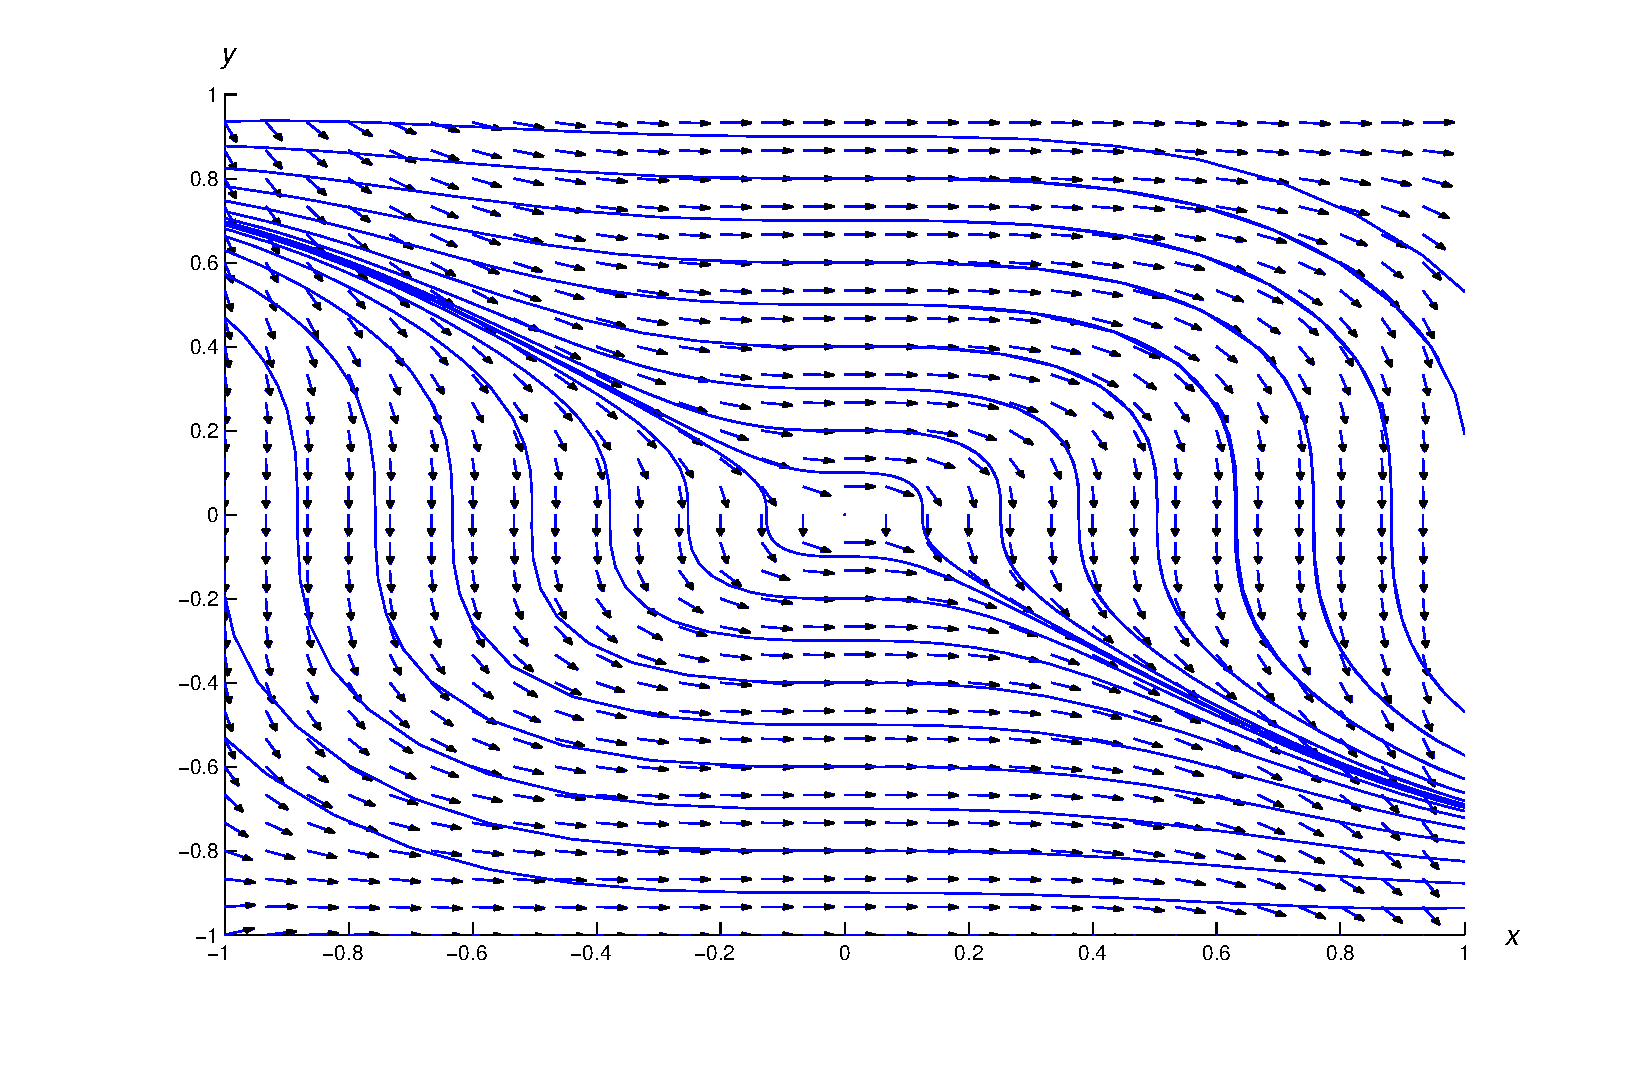
\includegraphics[bb=-78 148 689 643,width=5.67in,height=3.66in,keepaspectratio]{fig020501}
\color{blue}
\caption{A direction field and  integral curves for
$(4x^3y^3+3x^2)\,dx+(3x^4y^2+6y^2)\,dy=0$}
  \label{figure:2.5.1}
\end{figure}

Here's a summary of the procedure used in Method 1 of this
example. You should summarize procedure used in Method~2.

\smallskip
\color{blue}
\centerline{{\bf Procedure For Solving An Exact
Equation}}

\begin{description}
\item{\bf Step 1.} Check that the equation
\begin{equation} \label{eq:2.5.19}
 M(x,y)\,dx+N(x,y)\,dy=0
\end{equation}
satisfies the exactness condition  $M_y=N_x$. If not,
don't go further with this procedure.
\item{\bf Step 2.} Integrate
$$
{\partial F(x,y)\over\partial x}=M(x,y)
$$
with respect to $x$ to obtain
\begin{equation} \label{eq:2.5.20}
F(x,y)=G(x,y)+\phi(y),
\end{equation}
where $G$ is an antiderivative of $M$ with respect to $x$, and $\phi$
is an unknown function of $y$.
\item{\bf Step 3.} Differentiate \eqref{eq:2.5.20} with respect to
$y$  to obtain
$$
{\partial F(x,y)\over\partial y}={\partial G(x,y)\over\partial
y}+\phi'(y).
$$
\item{\bf Step 4.} Equate the right side of this equation to $N$ and solve
for $\phi'$;    thus,
$$
 {\partial G(x,y)\over\partial y}+\phi'(y)=N(x,y),\mbox{\quad  so \quad }
\phi'(y)=N(x,y)-{\partial G(x,y)\over\partial y}.
$$
\item{\bf Step 5.} Integrate $\phi'$ with respect to $y$, taking the
constant of integration to be zero, and substitute the result in
\eqref{eq:2.5.20} to obtain $F(x,y)$.
\item{\bf Step 6.} Set $F(x,y)=c$ to obtain an implicit solution of
\eqref{eq:2.5.19}. If possible, solve for $y$ explicitly as a
function of $x$.
\end{description}
\color{black}

It's a common mistake to omit Step 6. However, it's important to
include this step, since $F$ isn't  itself a solution of
\eqref{eq:2.5.19}.

Many equations can be conveniently solved by either of the two methods
used in Example~\ref{example:2.5.3}. However, sometimes the integration
required in one approach is  more difficult than in the
other. In such cases we choose the approach that requires the easier
integration.

\begin{example}\label{example:2.5.4} \rm
 Solve the equation
\begin{equation}  \label{eq:2.5.21}
(ye^{xy} \tan x+e^{xy} \sec^2x)\,dx+xe^{xy} \tan x\,dy=0.
\end{equation}
\end{example}

\solution We leave it to you to check that
$M_y=N_x$ on any open rectangle  where $\tan x$ and $\sec x$ are
defined. Here we must find a function $F$ such that
\begin{equation} \label{eq:2.5.22}
F_x(x,y)=ye^{xy} \tan x+e^{xy} \sec^2 x
\end{equation}
 and
\begin{equation}  \label{eq:2.5.23}
F_y(x,y)=xe^{xy} \tan x.
\end{equation}
 It's difficult to integrate \eqref{eq:2.5.22} with respect to $x$, but
easy to integrate \eqref{eq:2.5.23} with respect to $y$.  This yields
\begin{equation} \label{eq:2.5.24}
F(x,y)=e^{xy} \tan x+\psi (x).
\end{equation}
Differentiating this with respect to $x$ yields
$$
F_x(x,y)=ye^{xy}\tan x+e^{xy}\sec^2x+\psi'(x).
$$
 Comparing this with \eqref{eq:2.5.22} shows that  $\psi'(x)=0$.
Hence, $\psi$ is  a constant, which we can take to be zero in
\eqref{eq:2.5.24}, and
$$
e^{xy} \tan x=c
$$
is an implicit solution of \eqref{eq:2.5.21}. \bbox

Attempting to apply our procedure to an equation that isn't  exact
will lead to failure in  Step 4, since the function
$$
 N-{\partial G\over\partial y}
$$
won't be independent of $x$ if $M_y\ne N_x$
(Exercise~\ref{exer:2.5.31}), and therefore
can't be the derivative of a function of $y$ alone. Here's an example that
illustrates this.

\begin{example}\label{example:2.5.5}  \rm
 Verify that the equation
\begin{equation} \label{eq:2.5.25}
3x^2y^2\,dx+6x^3y\,dy=0
\end{equation}
is not exact, and show  that the procedure for solving exact equations
  fails when applied to \eqref{eq:2.5.25}.
\end{example}

\solution   Here
$$
M_y(x,y)=6x^2y \mbox{\quad  and \quad } N_x(x,y)=18x^2y,
$$
so \eqref{eq:2.5.25} isn't  exact. Nevertheless,  let's try to find
a function $F$ such that
\begin{equation} \label{eq:2.5.26}
F_x(x,y)=3x^2y^2
\end{equation}
and
\begin{equation} \label{eq:2.5.27}
F_y(x,y)=6x^3y.
\end{equation}
Integrating \eqref{eq:2.5.26} with respect to $x$ yields
$$
F(x,y)=x^3y^2+\phi(y),
$$
and differentiating this with respect to $y$ yields
$$
F_y(x,y)=2x^3y+\phi'(y).
$$
For this equation to be consistent with \eqref{eq:2.5.27},
$$
6x^3y=2x^3y+\phi'(y),
$$
or
$$
\phi'(y)=4x^3y.
$$
This is a contradiction, since $\phi'$  must be independent
of $x$. Therefore the procedure fails.

\exercises
In Exercises~\ref{exer:2.5.1}--\ref{exer:2.5.17} determine which equations
are exact and solve them.

\begin{exerciselist}
\item\label{exer:2.5.1}
$6x^2y^2\,dx+4x^3y\,dy=0$

\item\label{exer:2.5.2}
$(3y\cos x+4xe^x+2x^2e^x)\,dx+(3\sin x+3)\,dy=0$

\item\label{exer:2.5.3}
$14x^2y^3\,dx+21 x^2y^2\,dy=0$

\item\label{exer:2.5.4}
$(2x-2y^2)\,dx+(12y^2-4xy)\,dy=0$

\begin{tabular}[t]{@{}p{168pt}@{}p{168pt}}
 \item\label{exer:2.5.5}$(x+y)^2\,dx+(x+y)^2\,dy=0$&
\item\label{exer:2.5.6}$(4x+7y)\,dx+(3x+4y)\,dy=0$
\end{tabular}

\item\label{exer:2.5.7}
$(-2y^2\sin x+3y^3-2x)\,dx+(4y\cos x+9xy^2)\,dy=0$

\item\label{exer:2.5.8}
$(2x+y)\,dx+(2y+2x)\,dy=0$

\item\label{exer:2.5.9}
$(3x^2+2xy+4y^2)\,dx+(x^2+8xy+18y)\,dy=0$

\item\label{exer:2.5.10}
$(2x^2+8xy+y^2)\,dx+(2x^2+xy^3/3)\,dy=0$

\item\label{exer:2.5.11}
$\dst{\left({1\over x}+2x\right)\,dx+
\left({1\over y}+2y\right)\,dy=0}$

\item\label{exer:2.5.12}
$(y\sin xy+xy^2\cos xy)\,dx+(x\sin xy+xy^2\cos xy)\,dy=0$

\item\label{exer:2.5.13}
$\dst{{x\,dx\over(x^2+y^2)^{3/2}}+{y\,dy
\over(x^2+y^2)^{3/2}}=0}$

\item\label{exer:2.5.14}
$\left(e^x(x^2y^2+2xy^2)+6x\right)\,dx+(2x^2ye^x+2)\,dy=0$

\item\label{exer:2.5.15}
$\left(x^2e^{x^2+y}(2x^2+3)+4x\right)\,dx+(x^3e^{x^2+y}-12y^2)\,dy=0$

\item\label{exer:2.5.16}
$\left(e^{xy}(x^4y+4x^3)+3y\right)\,dx+(x^5e^{xy}+3x)\,dy=0$

\item\label{exer:2.5.17}
$(3x^2\cos xy-x^3y\sin xy+4x)\,dx+(8y-x^4\sin xy)\,dy=0$

\exercisetext{In Exercises~\ref{exer:2.5.18}--\ref{exer:2.5.22} solve
the initial value problem.}

\item\label{exer:2.5.18}
$(4x^3y^2-6x^2y-2x-3)\,dx+(2x^4y-2x^3)\,dy=0,\quad y(1)=3$

\item\label{exer:2.5.19}
$(-4y\cos x+4\sin x\cos x+\sec^2x)\,dx+
(4y-4\sin x)\,dy=0,\quad y(\pi/4)=0$

\item\label{exer:2.5.20}
$(y^3-1)e^x\,dx+3y^2(e^x+1)\,dy=0,\quad y(0)=0$

\item\label{exer:2.5.21}
$(\sin x-y\sin x-2\cos x)\,dx+\cos x\,dy=0,\quad y(0)=1$

\item\label{exer:2.5.22}
$(2x-1)(y-1)\,dx+(x+2)(x-3)\,dy=0,\quad y(1)=-1$

\item\label{exer:2.5.23} \CGex
Solve the exact equation
$$
(7x+4y)\,dx+(4x+3y)\,dy=0.
$$
Plot a direction field and some integral curves for this equation on
the rectangle
$$
\{-1\le x\le1,-1\le y\le1\}.
$$

\item\label{exer:2.5.24} \CGex
Solve the exact equation
$$
e^x(x^4y^2+4x^3y^2+1)\,dx+(2x^4ye^x+2y)\,dy=0.
$$
Plot a direction field and some integral curves for this equation on
the rectangle
$$
\{-2\le x\le2,-1\le y\le1\}.
$$

\item\label{exer:2.5.25} \CGex
Plot a direction field and some integral curves for the exact equation
$$
(x^3y^4+x)\,dx+(x^4y^3+y)\,dy=0
$$
on the rectangle $\{-1\le x\le 1,-1\le y\le1\}$. (See
Exercise~\ref{exer:2.5.37}\part{a}).

\item\label{exer:2.5.26} \CGex
Plot a direction field and some integral curves for the exact equation
$$
(3x^2+2y)\,dx+(2y+2x)\,dy=0
$$
on the rectangle $\{-2\le x\le 2,-2\le y\le2\}$. (See
Exercise~\ref{exer:2.5.37}(b)).

\item\label{exer:2.5.27} \Lex
\begin{alist}
\item % (a)
Solve the exact equation
$$
(x^3y^4+2x)\,dx+(x^4y^3+3y)\,dy=0
\eqno{\rm(A)}
$$
implicitly.
\item % (b)
For what choices of $(x_0,y_0)$ does
Theorem~\ref{thmtype:2.3.1} imply that the initial value problem
$$
(x^3y^4+2x)\,dx+(x^4y^3+3y)\,dy=0,\quad y(x_0)=y_0,
\eqno{\rm(B)}
$$
has a unique solution on an open interval $(a,b)$  that contains $x_0$?
\item % (b)
Plot a direction field and some integral curves for (A)
on a rectangular region centered at the origin. What is the
 interval of validity of the solution of (B)?
\end{alist}

\item\label{exer:2.5.28} \Lex
\begin{alist}
\item % (a)
Solve the exact equation
$$
(x^2+y^2)\,dx+2xy\,dy=0
\eqno{\rm(A)}
$$
implicitly.
\item % (b)
For what choices of $(x_0,y_0)$ does
Theorem~\ref{thmtype:2.3.1} imply that the initial value problem
$$
(x^2+y^2)\,dx+2xy\,dy=0,\quad y(x_0)=y_0,
\eqno{\rm(B)}
$$
has a unique solution $y=y(x)$ on some open interval $(a,b)$
that contains $x_0$?
\item % (c)
Plot a direction field and some integral curves for (A). From
the plot determine,
the  interval $(a,b)$ of \part{b}, the monotonicity
properties (if any) of the solution of (B), and $\lim_{x\to
a+}y(x)$ and $\lim_{x\to b-}y(x)$. \hint{Your answers will
depend upon which quadrant contains $(x_0,y_0)$.}
\end{alist}

\item\label{exer:2.5.29}
Find all functions $M$ such that the  equation is exact.
\begin{alist}
\item %(a)
$M(x,y)\,dx+(x^2-y^2)\,dy=0$
\item %(b)
$M(x,y)\,dx+2xy\sin x\cos y\,dy=0$
\item %(c)
$M(x,y)\,dx+(e^x-e^y\sin x)\,dy=0$
\end{alist}

\item\label{exer:2.5.30}
Find all functions $N$ such that the  equation is exact.
\begin{alist}
\item %(a)
$(x^3y^2+2xy+3y^2)\,dx+N(x,y)\,dy=0$
\item %(b)
$(\ln xy+2y\sin x)\,dx+N(x,y)\,dy=0$
\item %(c)
$(x\sin x+y\sin y)\,dx+N(x,y)\,dy=0$
\end{alist}

\item\label{exer:2.5.31}
Suppose $M$, $N$, and their partial derivatives are continuous on
an open rectangle
$R$, and $G$ is an antiderivative of $M$ with respect to $x$; that is,
$$
{\partial G\over\partial x}=M.
$$
Show that if $M_y\ne N_x$ in $R$ then the function
$$
 N-{\partial  G\over\partial y}
$$
is not independent of $x$.

\item\label{exer:2.5.32}
Prove:  If the equations $M_1\,dx+N_1\,dy=0$ and $M_2\,
dx+N_2\,dy=0$ are exact on an open rectangle $R$,  so is
the equation $$(M_1+M_2)\,dx+(N_1+N_2)\,dy=0.$$

\item\label{exer:2.5.33}
Find conditions on the constants $A$, $B$, $C$, and $D$ such that
the equation
$$
(Ax+By)\,dx+(Cx+Dy)\,dy=0
$$
is exact.

\item\label{exer:2.5.34}
Find conditions on the constants $A$, $B$, $C$, $D$, $E$, and
$F$ such that the equation
$$
(Ax^2+Bxy+Cy^2)\,dx+(Dx^2+Exy+Fy^2)\,dy=0
$$
is exact.

\item\label{exer:2.5.35}
Suppose $M$ and $N$ are continuous and have continuous partial
derivatives $M_y$ and $N_x$ that satisfy the exactness condition
$M_y=N_x$ on an open rectangle $R$.
  Show that if $(x,y)$ is in $R$ and
$$
F(x,y)=\int^x_{x_0}M(s,y_0)\,ds+\int^y_{y_0}N(x,t)\,dt,
$$
then $F_x=M$ and $F_y=N$.

\item\label{exer:2.5.36}
Under the assumptions of Exercise~\ref{exer:2.5.35}, show that
$$
F(x,y)=\int^y_{y_0}N(x_0,s)\,ds+\int^x_{x_0}M(t,y)\,dt.
$$

\item\label{exer:2.5.37}
Use the method suggested by Exercise~\ref{exer:2.5.35}, with
$(x_0,y_0)=(0,0)$, to solve the these exact equations:
\begin{alist}
\item %(a)
$(x^3y^4+x)\,dx+(x^4y^3+y)\,dy=0$
\item %(b)
$(x^2+y^2)\,dx+2xy\,dy=0$
\item %(c)
$(3x^2+2y)\,dx+(2y+2x)\,dy=0$
\end{alist}

\item\label{exer:2.5.38}
Solve the initial value problem
$$
y'+{2\over x}y=-{2xy\over x^2+2x^2y+1},\quad y(1)=-2.
$$

\item\label{exer:2.5.39}
Solve the initial value problem
$$
y'-{3\over x}y={2x^4(4x^3-3y)\over3x^5+3x^3+2y},\quad y(1)=1.
$$

\item\label{exer:2.5.40}
Solve the initial value problem
$$
y'+2xy=-e^{-x^2}\left({3x+2ye^{x^2}\over2x+3ye^{x^2}}\right),\quad
y(0)=-1.
$$

\item\label{exer:2.5.41}
Rewrite the separable equation
$$
h(y)y'=g(x)
\eqno{\rm (A)}
$$
as an exact equation
$$
M(x,y)\,dx+N(x,y)\,dy=0.
\eqno{\rm (B)}
$$
Show that applying the method of this section  to
(B) yields the same solutions that would be
obtained by applying the method of separation of variables
to~(A)

\item\label{exer:2.5.42}
Suppose  all second partial derivatives of $M=M(x,y)$ and $N=N(x,y)$
are continuous and $M\,dx+N\,dy=0$ and $-N\,dx+M\,dy=0$ are
exact on an open rectangle  $R$.  Show that
$M_{xx}+M_{yy}=N_{xx}+N_{yy}=0$ on
$R$.

\item\label{exer:2.5.43} Suppose all second partial derivatives of
$F=F(x,y)$ are continuous and $F_{xx}+F_{yy}=0$ on an open rectangle
$R$. (A function with these properties is said to be {\color{blue}\it harmonic\/};
see also Exercise~\ref{exer:2.5.42}.) Show that $-F_y\,dx+F_x\,dy=0$ is
exact on $R$, and
therefore there's a function $G$ such that
$G_x=-F_y$ and $G_y=F_x$ in $R$. (A function $G$ with this property is
said to be a {\color{blue}\it harmonic conjugate\/} of $F$.)

\item\label{exer:2.5.44}
Verify that the following functions are harmonic, and find all their
harmonic conjugates.  (See Exercise~\ref{exer:2.5.43}.)

\begin{tabular}[t]{@{}p{112pt}@{}p{112pt}p{112pt}}
{\bf (a)}\   $x^2-y^2$
& {\bf (b)}\   $e^x\cos y$
& {\bf (c)}\   $x^3-3xy^2$\\
{\bf (d)}\   $\cos x\cosh y$
& {\bf (e)}\   $\sin x\cosh y$ &
\end{tabular}

\end{exerciselist}
